\documentclass[13pt]{beamer}

\usepackage{Handle}

\DeclareFontFamily{U}{BOONDOX-calo}{\skewchar\font=45}
\DeclareFontShape{U}{BOONDOX-calo}{m}{n}{
  <-> s*[1.05] BOONDOX-r-calo}{}
\DeclareMathAlphabet{\mathcalboondox}{U}{BOONDOX-calo}{m}{n}
\newcommand{\bondox}{\mathcalboondox}

\newcommand{\Title}{Two betweenness centrality
measures based on Randomized
Shortest Paths}
\newcommand{\Subtitle}{Prova Integrativa - Complessità nei Sistemi e nelle Reti}
\newcommand{\YourName}{Matteo Bonfadini}
\newcommand{\Institute}{ Politecnico di Milano}
\newcommand{\ImageUrl}{Images/graph.jpg}

\begin{document}
    \begin{frame}[noframenumbering,plain,t]

        \begin{tikzpicture}[remember picture, overlay]
            \node[opacity = 0.8] at (current page.center)
            {
                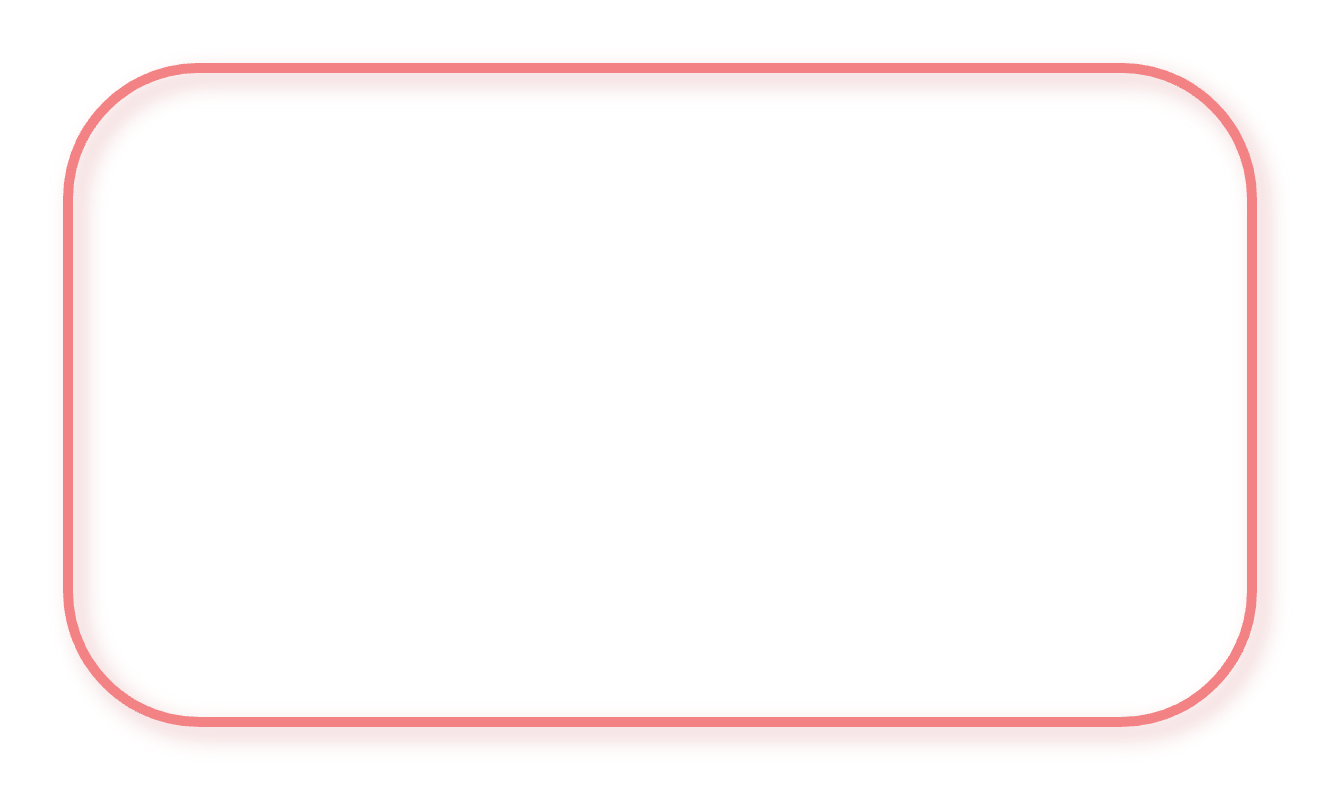
\includegraphics[height = 0.75\paperwidth, width = 1\paperwidth]{Images/bg9.png}
            };
        \end{tikzpicture}

        \MakeTitle

    \end{frame}


    \begin{frame}{Outline}
        \begin{tikzpicture}[remember picture, overlay]
            \node[opacity = 0.2] at (current page.center)
            {
                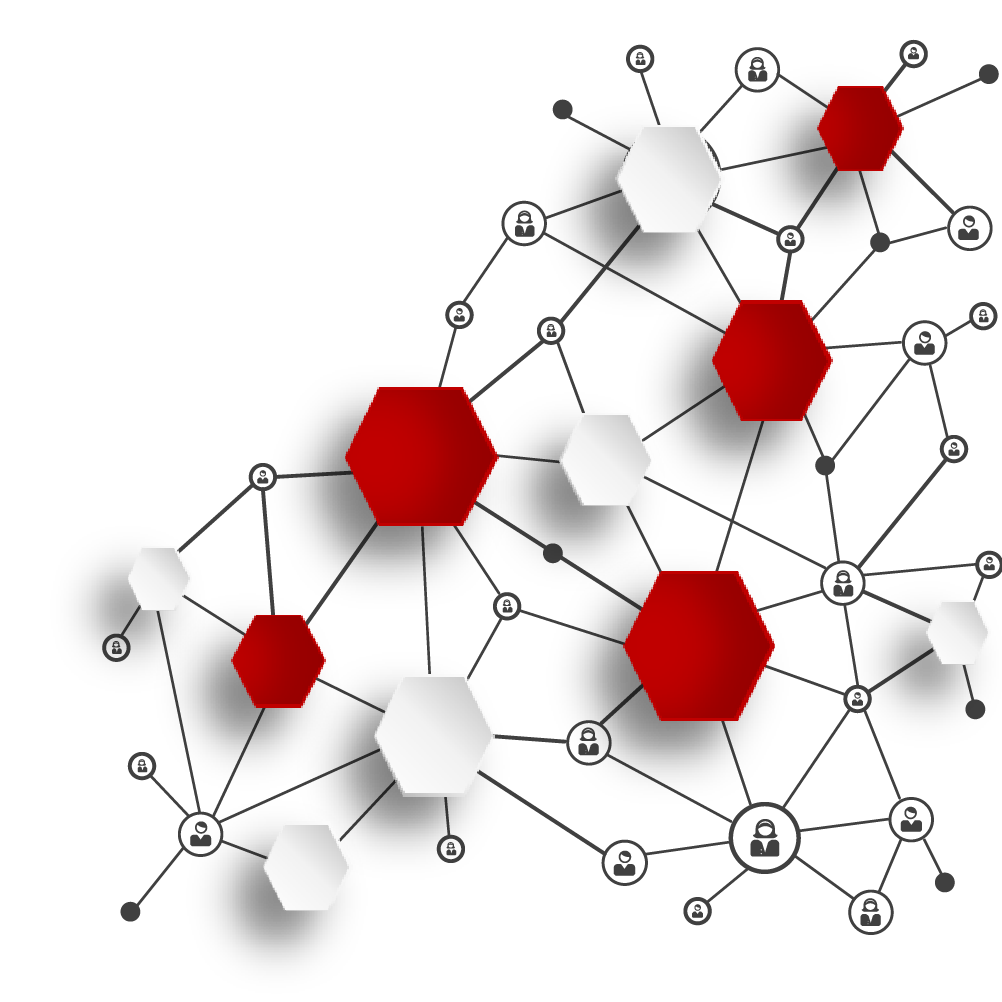
\includegraphics[height = 0.75\paperwidth]{Images/bg3.png}
            };
        \end{tikzpicture}

        \normalsize
        \tableofcontents
    \end{frame}

    \section{Goal}

    \begin{frame}[t,allowframebreaks]{RSP framework}
    One of the most fundamental topics in network science is determining the \emph{centrality} of a node in a network accordingly to its structure. The concept of centrality can be interpreted in many ways and a vast number of measures have been proposed.\\
    \vspace{0.8em}
    We aim to introduce two new closely related betweenness centrality measures based on the Randomized Shortest Paths (RSP) framework:
    \begin{itemize}
        \item the simple RSP betweenness

        \item the RSP net betweenness
    \end{itemize}

    \newpage

    The RSP framework is based on \emph{Boltzmann probability distributions} over paths between the nodes of a network which focus on short, optimal paths, but give some probablity mass also to longer paths.\\
    \vspace{0.8em}
    The Boltzmann probabilities describe the probability that a thermodynamic system is in a particular state, given a certain \emph{energy} value of that system.\\
    \vspace{0.8em}
    Rather than the energy, we'd like to control the focus on optimal paths with an inverse temperature parameter $\beta$.
    \end{frame}

    \begin{frame}[t,allowframebreaks]{Usefulness}
    Measures based only on shortest paths or random walks alone often involve undesirable features:
    \begin{itemize}
        \item highly skewed betweenness score distribution in complex networks;

        \item not always realistic to consider that navigating agents would occur along only the shortest paths;

        \item random walks may depend heavely on local features of a graph, especially for large graphs.
    \end{itemize}

    \newpage

    Because of this, RSP's measures can help:
    \begin{itemize}
        \item in detecting bottlenecks of the networks, where there exist no alternatives for the shortest path;

        \item in introducing some regularisation over the degree of randomness, which is controlled by the inverse temperature parameter $\beta$.
    \end{itemize}
    \vspace{0.8em}
    In addiction, the RSP framework has previously been used for defining distance measures in many data analysis tasks such as clustering and classification of graph nodes.
    \end{frame}

    \section{RSP betweenness centralities}

    \begin{frame}[t,allowframebreaks]{Notation and terminology}

        \begin{itemize}
            \item  We consider weighted directed graphs $G=(V,E)$ with node set $V=\{1,2,\dots,n\}$ and edge set $E=\{(i,j)\}$ of $m$ edges.

            \item Each edge of the graph is associated with a \textbf{weight} $a_{ij}$ and a \textbf{cost} $c_{ij}$:

            \begin{itemize}
                \item The weights are collected in the non-symmetric $n\times n$ \emph{adjacency matrix} $\mathbf{A}$ and they reflect the strength of connection between adjacent nodes.

                \item The edge weights define the \emph{reference transition probability matrix} $\mathbf{P}^{\text{ref}}$, which can be computed as
                \begin{equation*}
                \mathbf{P}^{\text{ref}}=\mathbf{D}^{-1}\mathbf{A},\qquad\mathbf{D}=\text{diag}(k_1,\dots,k_n)
                \end{equation*}
                or
                \begin{equation*}
                p^{\text{ref}}_{ij} = \frac{a_{ij}}{\sum_{j} a_{ij}} = \frac{a_{ij}}{s_i^{\text{out}}}
                \end{equation*}

                \item The edge costs, in contrast to weights, describe the distance of adjacent nodes. The cost of a path $\bondox{P}$ is
                \begin{equation*}
                \widetilde{c}(\bondox{P})=\sum_{(i,j)\in\bondox{P}} c_{ij}
                \end{equation*}
            \end{itemize}

        \end{itemize}

        In many situations the edge costs and edge weights can be defined based on one another, for istance, as $c_{ij}=1/a_{ij}$. 

        However, in the RSP framework the weights can be independent of the costs, thus the transition probabilities do not depend on the costs. This means that:

        \begin{itemize}
            \item[$\triangleright$] the edge costs define the interpretation of shortest paths, i.e. the \emph{low temperature behavior} of the system;

            \item[$\triangleright$] the edge weights determine the interpretation of a random walk, i.e. the \emph{high temperature behavior}.
        \end{itemize}

    \end{frame}

    \begin{frame}[t,allowframebreaks]{Minimization of expected cost}

    For semplicity, we restrict the RSP framework to absorbing paths (for istance, take a directed strongly connected network).\\
    \vspace{0.8em}
    The RSP framework is based on the probability distribution over the set $\mathcal{P}_{st}$ of absorbing $s$-$t$-walks for which the expected cost of the walk is minimal when constrained with a fixed relative entropy w.r.t. the reference path probability distribution. Formally, we seek for the solution to the following problem:
    \begin{equation*}
    \min_{\widetilde{P}_{st}}\sum_{\bondox{P}\in \mathcal{P}_{st}}\widetilde{P}_{st}(\bondox{P})\,\widetilde{c}(\bondox{P})\quad\text{s.t.}\quad \begin{cases}
    J\left(\widetilde{P}_{st}||\widetilde{P}_{st}^{\text{ref}}\right)=J_0 \\
    \displaystyle \sum_{\bondox{P}\in \mathcal{P}_{st}} \widetilde{P}_{st}(\bondox{P}) = 1
    \end{cases}
    \end{equation*}

    The solution is a Boltzmann distribution:
    \begin{equation*}
    \widetilde{P}_{st}(\bondox{P})=\frac{\widetilde{P}_{st}^{\text{ref}}(\bondox{P})\,e^{-\beta\widetilde{c}(\bondox{P})}}{\mathcal{Z}_{st}} 
    \end{equation*}
    where
    \begin{equation*}
    \mathcal{Z}_{st}=\sum_{\bondox{P}\in \mathcal{P}_{st}}\widetilde{P}_{st}^{\text{ref}}(\bondox{P})\,e^{-\beta\widetilde{c}(\bondox{P})}
    \end{equation*}
    is the \emph{partition function} of absorbing $s$-$t$-walks. 
    \end{frame}

    \begin{frame}[t,allowframebreaks]{Matrix formulation}
    Concerning the computation of $\mathcal{Z}_{st}$, we have that
    \begin{equation*}
    \mathcal{Z}_{st}=\frac{z_{st}}{z_{tt}} 
    \end{equation*}
    where $z_{st}$ is the $(s,t)$-element of the \emph{fundamental matrix of non-absorbing paths}
    \begin{equation*}
    \mathbf{Z}=(\mathbf{I}-\mathbf{W})^{-1}\quad\text{with}\quad \mathbf{W}=\mathbf{P}^{\text{ref}}\circ e^{-\beta\mathbf{C}}
    \end{equation*}
    
    The matrix $\mathbf{W}$ is a substochastic matrix and can be interpreted as defining a \emph{killed random walk}. Hence, one can see the partition function $\mathcal{Z}_{st}$ as the probability of a walker surviving the walk from $s$ to $t$.
    \end{frame}

    \begin{frame}[t,allowframebreaks]{Simple RSP betweenness}
    The simple RSP betweenness centrality of a node $i$ is
    \begin{equation*}
    \text{bet}_i^{\text{RSP}}=\sum_{s,t=1}^n \text{bet}_i^{\text{RSP}}(s,t)
    \end{equation*}
    where $\text{bet}_i^{\text{RSP}}(s,t)$ is the RSP simple betweenness of the node $i$ w.r.t. absorbing paths from $s$ to $t$, i.e. the expected number of visits through $i$ over all $s$-$t$-walks w.r.t. the RSP solution probabilities:
    \begin{equation*}
    \text{bet}_i^{\text{RSP}}(s,t)=
    \begin{cases}
    0 &\text{if }\nexists\ s\text{-}t\text{-path}\\
    \displaystyle\sum_{j=1}^n\overline{\eta}_{ij}(s,t) &\text{otherwise}
    \end{cases}
    \end{equation*} 
    where 
    \begin{equation*}
    \overline{\eta}_{ij}(s,t)=-\frac{1}{\beta}\,\frac{\partial\log \mathcal{Z}_{st}}{\partial c_{ij}}=-\frac{1}{\beta}\,\frac{\partial\log\left(z_{st}/z_{tt}\right) }{\partial c_{ij}}=\left(\frac{z_{si}}{z_{st}}-\frac{z_{ti}}{z_{tt}}\right)w_{ij}z_{jt}
    \end{equation*}
    In other words, the total flow transiting through node $i$ is
    \begin{equation*}
    \text{bet}_i^{\text{RSP}}(s,t)=\underbracket[0.5pt]{\left(\frac{z_{si}}{z_{st}}-\frac{z_{ti}}{z_{tt}}\right)}_{=0\text{ if }i=t}\underbracket[0.5pt]{\sum_{j} w_{ij}z_{jt}}_{\begin{gathered}
    \scriptstyle{=z_{it}\text{ if }i\neq t} \\
    \scriptstyle{\mathbf{Z}=(\mathbf{I}-\mathbf{W})^{-1}} \\
    \scriptstyle{\mathbf{Z}(\mathbf{I}-\mathbf{W})=\mathbf{I}} \\
    \scriptstyle{\mathbf{Z}=\mathbf{ZW}+\mathbf{I}} \\
    \end{gathered}}=\left(\frac{z_{si}}{z_{st}}-\frac{z_{ti}}{z_{tt}}\right)z_{it}
    \end{equation*}

    Finally, the simple RSP betweenness of node $i$ is
    \begin{align*}
    \text{bet}_i^{\text{RSP}}&=\sum_{s,t}\text{bet}_i^{\text{RSP}}(s,t)=\\
    &=\sum_{s,t} \left(\frac{z_{si}}{z_{st}}-\frac{z_{ti}}{z_{tt}}\right)z_{it}=\\
    &=\left[ \textbf{diag}\left( \mathbf{Z} \left(\mathbf{Z}^\div-n \textbf{Diag}\left( \mathbf{Z}^\div \right) \right)^T\mathbf{Z} \right) \right]_i
    \end{align*}

    The vector $\textbf{bet}^\text{RSP}$ of all betweenness values is computed accordingly.
    \end{frame}

    \begin{frame}[t,allowframebreaks]{Computing the simple RSP betweenness}
    \textbf{Input:}
    \begin{itemize}
        \item a directed strongly connected graph $G$ with $n$ nodes
        \item the $n\times n$ reference transition probability matrix $\mathbf{P}^\text{ref}=\mathbf{D}^{-1}\mathbf{A}$
        \item the $n\times n$ cost matrix $\mathbf{C}$
        \item the inverse temperature parameter $\beta$
    \end{itemize}

    \textbf{Output:}
    \begin{equation*}
    \begin{array}{cl}
    1. & \mathbf{W}=\mathbf{P}^\text{ref}\circ e^{-\beta\mathbf{C}} \\
    2. & \mathbf{Z}=(\mathbf{I}-\mathbf{W})^{-1} \\
    3. & \mathbf{Z}^\div=\mathbf{e}\mathbf{e}^T\div\mathbf{Z} \\
    4. & \text{return }\textbf{bet}^\text{RSP}=\textbf{diag}\left( \mathbf{Z} \left(\mathbf{Z}^\div-n \textbf{Diag}\left( \mathbf{Z}^\div \right) \right)^T\mathbf{Z} \right)
    \end{array}
    \end{equation*}

    This highlight the computational bottleneck of the algorithm: the matrix inversion, which, in general, has complexity $\mathcal{O}\left( n^3 \right)$.
    \end{frame}

    \begin{frame}[t,allowframebreaks]{RSP net betweenness}
    Instead of only considering the overall outgoing flow of random walkers it may in some cases make more sense to compute the net outgoing flow, i.e. so that the outgoing and ingoing flows through one edge neutralize each other. This corresponds to the random walk interpretation of the \emph{current flow betweenness} in undirected graphs.\\
    \vspace{0.8em} 
    According to this approach, we define the \emph{RSP net betweenness centrality} of node $i$ as
    \begin{equation*}
    \text{bet}_i^{\text{RSPnet}}=\sum_{s,t}
    \sum_{j}\left|\overline{\eta}_{ij}(s,t)-\overline{\eta}_{ji}(s,t)\right|
    \end{equation*}

    \end{frame}

    \section{Limits and Experiments}

    \begin{frame}[t,allowframebreaks]{Limits}
    \begin{equation*}
    \widetilde{P}_{st}(\bondox{P})=\frac{\widetilde{P}_{st}^{\text{ref}}(\bondox{P})\,e^{-\beta\widetilde{c}(\bondox{P})}}{\mathcal{Z}_{st}},\qquad 
    \mathcal{Z}_{st}=\sum_{\bondox{P}\in \mathcal{P}_{st}}\widetilde{P}_{st}^{\text{ref}}(\bondox{P})\,e^{-\beta\widetilde{c}(\bondox{P})}
    \end{equation*}
    
    \begin{itemize}
        \item At the limit $\beta\to\infty$. In the low temperature limit, the RSP probability distribution focuses solely on shortest paths. Thus 
        \begin{equation*}
        \widetilde{P}_{st}(\bondox{P})\xrightarrow{\beta\to\infty}\begin{cases}
            0, &\ \text{ if }\bondox{P}\notin \mathcal{P}^*_{st}\\
            \dfrac{\widetilde{P}_{st}^{\text{ref}}(\bondox{P})}{\displaystyle \sum_{\bondox{P}\in\mathcal{P}^*_{st}} \widetilde{P}_{st}^{\text{ref}}(\bondox{P})} &\ \text{ if }\bondox{P}\in \mathcal{P}^*_{st}
        \end{cases}
        \end{equation*}

        In other words, the simple RSP  betweenness converges to the \emph{shortest path likelihood betweenness}.

        The same result holds for the RSP net betweenness. Intuitively, as the path distribution focuses more and more on the shortest paths, one of the two terms of in and outgoing flows becomes zero, as the walker will only move in one direction.

        \item At the limit $\beta\to0^+$. In the high temperature limit the RSP probabilities converge to the \emph{unbiased random walk probabilities}, determined by the reference transition probabilities, i.e.
        \begin{equation*}
        \widetilde{P}_{st} \xrightarrow{\beta\to0^+}\widetilde{P}_{st}^{\text{ref}}\qquad\forall\, \bondox{P}
        \end{equation*}
        This means that the simple RSP betweenness is proportional to the stationary distribution $\pi$ s.t. $\pi=\left( \mathbf{P}^\text{ref} \right)^T\pi$.
    \end{itemize}

    \end{frame}

    \begin{frame}[t,allowframebreaks]{Artificial example}
    One possible use for the RSP betweenness measures is the detection of groups of nodes that are central in a network.

    \begin{figure}
    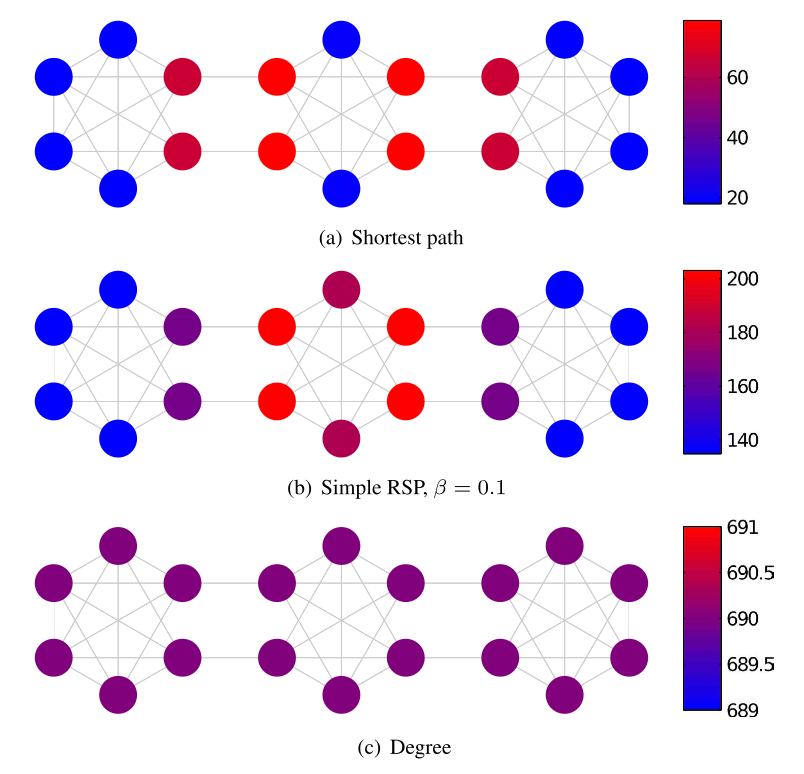
\includegraphics[height =0.6\paperheight]{Images/heat1.png}
    \end{figure}
    \end{frame}

    \begin{frame}[t,allowframebreaks]{Manhattan street network.}
    One promising application area for RSP’s are path planning problems.

    \vspace{0.8em}

    We illustrate the use of RSP’s for routing in a network by analyzing the street network of Midtown and Lower Manhattan.

    \begin{center}
    \begin{figure}
    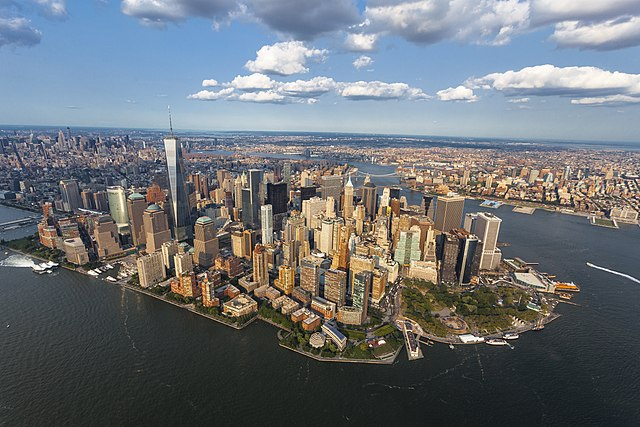
\includegraphics[height=0.4\paperheight]{Images/man.jpg}
    \end{figure}
    \end{center}

    \newpage

    The nodes in the network correspond to intersections and the edges are the street segments between the intersections; we treat the network as undirected. 

    \vspace{0.8em}

    The length of each street segment is assigned as the cost of the corresponding edge. Accordingly, the overall
    cost of a path is its overall length. However, we define here the reference transition probabilities of the random
    walk according to the degree of each node, $p_{ij}^\text{ref}=1/k_i$, i.e. only according to the number of edges connected to the node and independent of the edge costs.

    \newpage

    \begin{center}
    \begin{figure}
    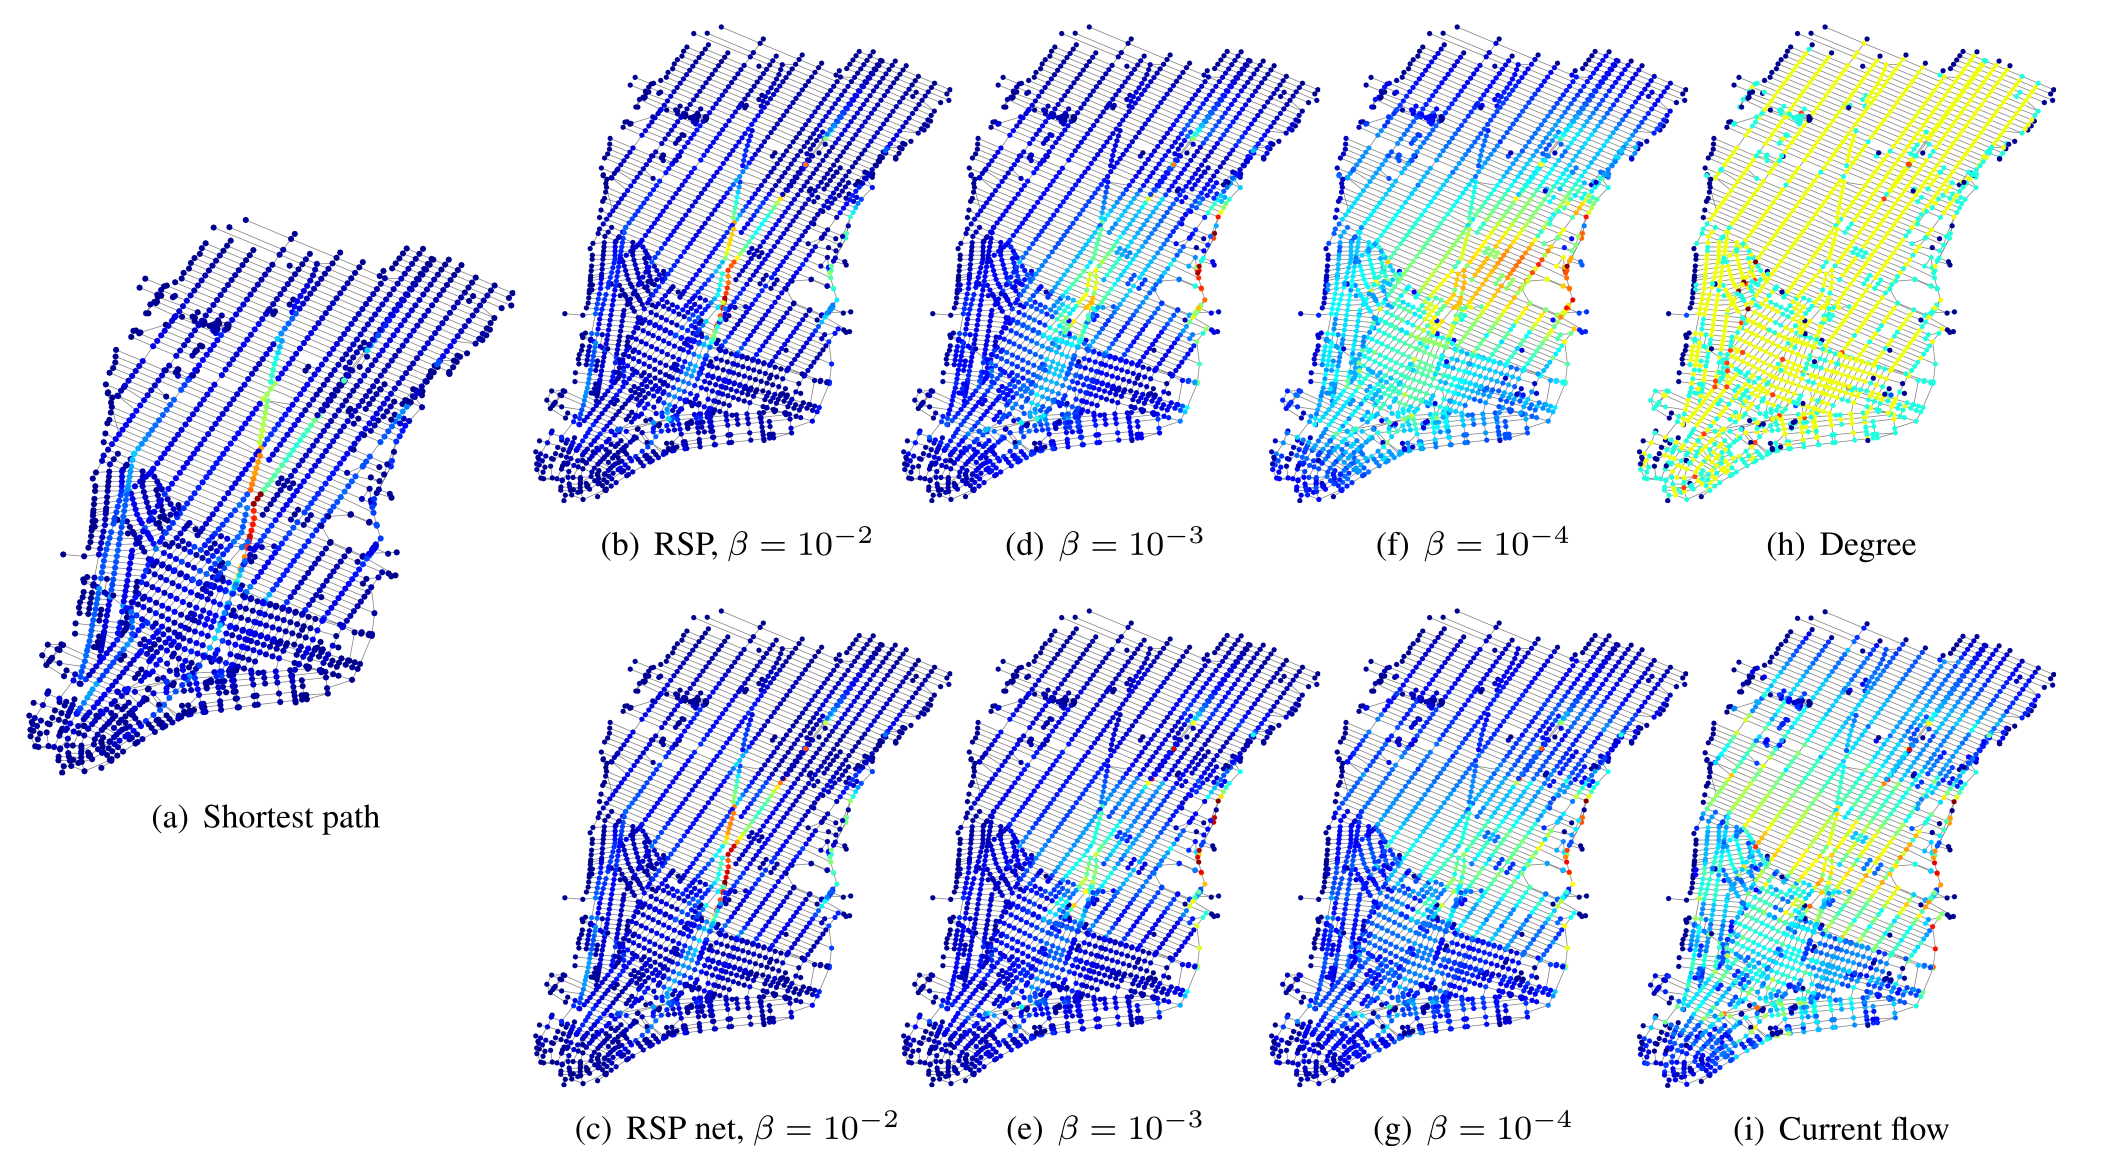
\includegraphics[height=0.65\paperheight]{Images/heat2.png}
    \end{figure}
    \end{center}

    \end{frame}

    % \section{Old}

    % \setbeamercolor{section in head/foot}{bg=cyan,fg=black}
    % \setbeamercolor{frametitle}{bg=aqua,fg=black}
    % \setbeamercolor{author in head/foot}{bg=aqua,fg=black}

    % \begin{frame}[t,allowframebreaks]{Types of Graph}
    %     \begin{columns}
    %         \column{0.5\textwidth}
    %         \begin{bee}[Undirected Graph,width = 6cm]{black}{aqua}
    %             A graph in which edges do not have any direction.
    %         \end{bee}
    %         \column{0.55\textwidth}
    %         \begin{Rbee}[Directed Graph,width = 6cm]{arsenic}{aqua}
    %             A graph in which edge has direction.
    %         \end{Rbee}
    %     \end{columns}
    %     \begin{figure}
    %             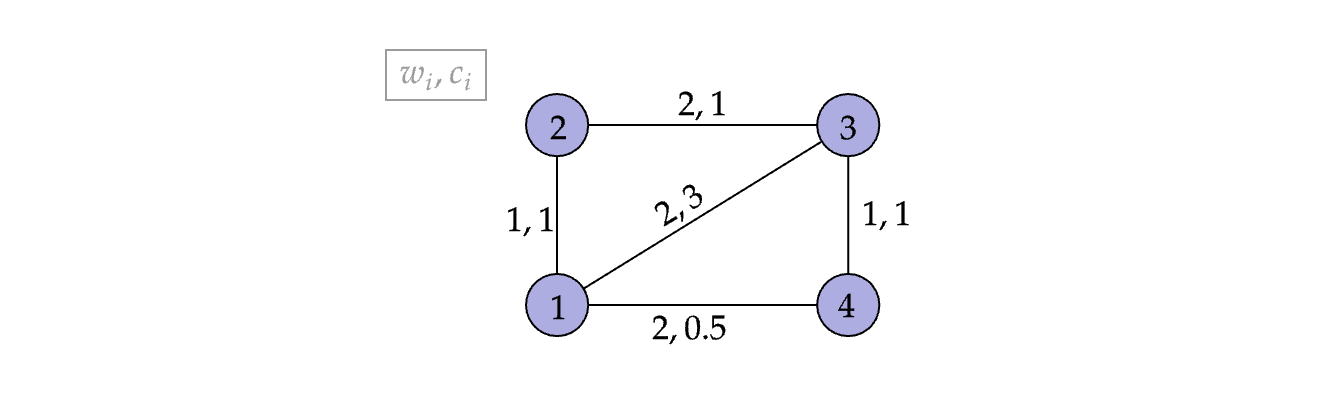
\includegraphics[height =0.4\paperheight]{Images/diagram-20240216.png}
    %     \end{figure}


    %     \begin{bee}[Complete Graph,width = 8cm]{white}{deepmagenta}
    %         A graph in which every pair of distinct nodes is connected by an edge
    %     \end{bee}
    %        \vspace{-5mm}
    %     \begin{Rbee}[Forest,width = 0.86\paperwidth]{white}{arsenic}
    %         A collection of trees or disjoint tree-like structures within a graph
    %     \end{Rbee}
    %     \begin{bee}[Tree,width = 0.9\paperwidth]{white}{blue}
    %         A special case of an acyclic graph in which there is a single root node, and every other node is connected by exactly one edge.
    %     \end{bee}

    % \end{frame}

    % \begin{frame}[t,allowframebreaks]{Introduction to Graphs}

    % \begin{itemize}
    %     \item  A Graph is a non-linear data structure consisting of vertices and edges.
    %     \item The \textbf{Vertices} are sometimes also referred to as nodes and the \textbf{Edges} are lines or arcs that connect any two nodes in the graph.

    %     \begin{bee}[More formally]{white}{arsenic}
    %         A Graph is composed of a set of vertices V and a set of edges E. \\
    %         The graph is denoted by \textbf{G(V,E)}.
    %     \end{bee}

    % \end{itemize}

    % \end{frame}

\end{document}
